\documentclass[11pt]{article}

\usepackage{fancyhdr}
\usepackage{amsmath}
\usepackage{graphicx}
\usepackage{float}
\usepackage[top=1in, bottom=1in, left=.5in, right=.5in]{geometry}
%\usepackage[font=small,labelfont=bf]{caption}

% Title.
% ------
\title{STAT 240 Homework 1}
\author{Rebecca Barter, Andrew Do and Kellie Ottoboni}



\begin{document}

\maketitle

 
 \section*{Question 1. Consider a box that contains 5 ``1'' tickets and 7 ``0'' tickets. Consider drawing 6 tickets from this box at random with replacement. Let $X_1, X_2, ..., X_6$ denote the 6 numbers you observe. Let $\bar{X}$ denote the average of the draws.}
 
 \subsection*{a) What is $E[\bar{X}]$?}
 \vspace{5mm}
 \noindent Recall that in class we showed that
 \begin{align*}
 E(\bar{X}) &= \bar{t}
 \end{align*}
 
 \noindent where $\bar{t}$ is the population mean. In particular, this implies that
 
\begin{align*}
E(\bar{X})= \frac{5}{12}
 \end{align*}
 
 
 \vspace{5mm}
 \subsection*{b) What is $SE[\bar{X}]$? (R hint: Be careful whether the function ``sd'' divides by the square root of $n$ or $n - 1$)}
  \vspace{5mm}
 \noindent Note that since this example corresponds to a simple box model with replacement, we have that
 $$SE(\bar{X}) = \sqrt{Var(\bar{X})} = \sqrt{\frac1n Var(t)}$$
 
 
 \noindent Using R and noting that the \texttt{sd()} function in R divides by $N-1$ rather than $N$, we found that (to 3dp)
 $$SE(\bar{X}) = 0.201$$
 

  \vspace{5mm}
 \subsection*{c) Use R to simulate 100,000 values of $\bar{X}$. Produce a histogram of these values. (R hint: Use the function sample).}
 
 
 
\begin{figure}[H]
\centering
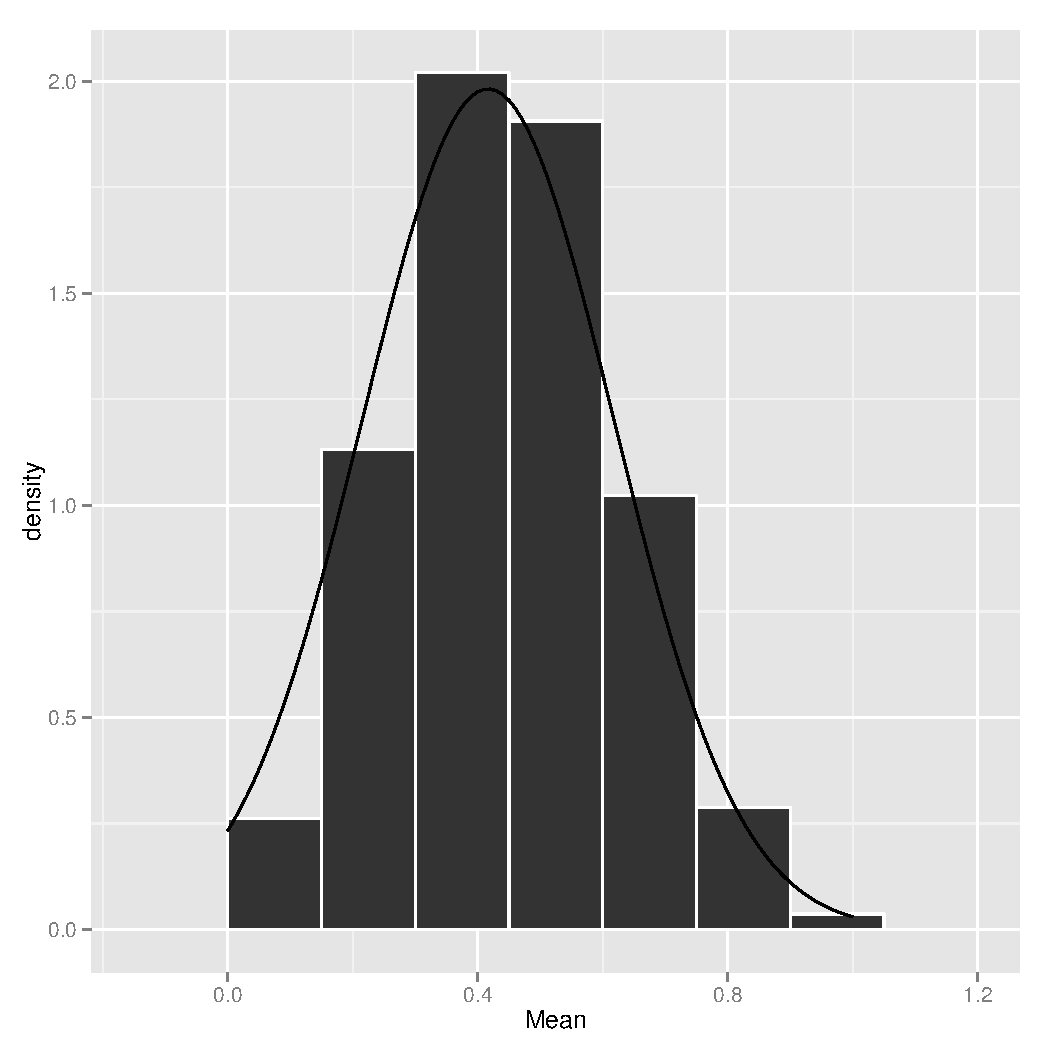
\includegraphics[width = .5\textwidth]{histogram_1c-1.pdf}
\caption{Histogram of 100,000 simulated values of the sample mean when the sample was taken with replacement from a box that contains 5 ``1'' tickets and 7 ``0'' tickets.}
\end{figure}
 
 \subsection*{d) Let $z_1 = E[\bar{X}] + SE[\bar{X}], ~ z_2 = E[\bar{X}] + 2 \times SE[\bar{X}]$, etc. For $z_1, ..., z_4$ calculate $P(\bar{X} > z_i)$ in three ways:
 \begin{itemize}
 \item Exactly, using the binomial distribution. (Hint: It will be easier to work with the sample sum than the sample average. R hint: Use function pbinom)
 \item Estimated using the values from part (c)
 \item Using the normal approximation. Use the continuity correction. (R hint: pnorm)
 \end{itemize}
 Do the same for $z_{-4},...,z_{-1}$ but calcualte $P(\bar{X} < z_i)$ instead of $P(\bar{X} > z_i)$. Make a table of your results and comment briefly}

\begin{table}[H]
\centering
\begin{tabular}{|c|ccc|}
  \hline
z & Exact & EmpiricalEst & NormalApprox \\ 
  \hline
-4.00 & 0.00 & 0.00 & 0.00 \\ 
  -3.00 & 0.00 & 0.00 & 0.00 \\ 
  -2.00 & 0.04 & 0.04 & 0.06 \\ 
  -1.00 & 0.21 & 0.21 & 0.28 \\ 
  1.00 & 0.20 & 0.20 & 0.28 \\ 
  2.00 & 0.05 & 0.05 & 0.06 \\ 
  3.00 & 0.00 & 0.00 & 0.00 \\ 
  4.00 & 0.00 & 0.00 & 0.00 \\ 
   \hline
\end{tabular}
\caption{The exact value, empirical estimation and normal approximation of the tail probability for a box that contains 5 ``1'' tickets and 7 ``0'' tickets.} 
\end{table}

\noindent We notice that the Empirical estimation using the results of our simulated value is extremely close the the exact value of the probabilities. On the other hand, the normal approximation is not nearly as accurate. This is likely because our sample size of 6 is very small and the asymptotic assumptions which underly the normal approximation are not yet accurate.



\subsection*{e) Repeat (a)-(d), this time sampling without replacement instead of with replacement. Use the hypergeometric distirbution instead of the binomial distribuion (R hint: phyper)}


\noindent Note that since we are now sampling without replacement, we still have that
$$E(\bar{X}) = \bar{t} = \frac{5}{12}$$

\noindent but now the SE is given by
$$SE(\bar{X}) = \sqrt{Var(\bar{X})} = \sqrt{\frac{1}{n} Var(t) \left[\frac{N - n}{N - 1}\right]} = 0.149$$

\noindent which is smaller than the SE when sampling with replacement.\\

\noindent Next, sampling 100,000 values of $\bar{X}$, we obtain the following histogram.

\begin{figure}[H]
\centering
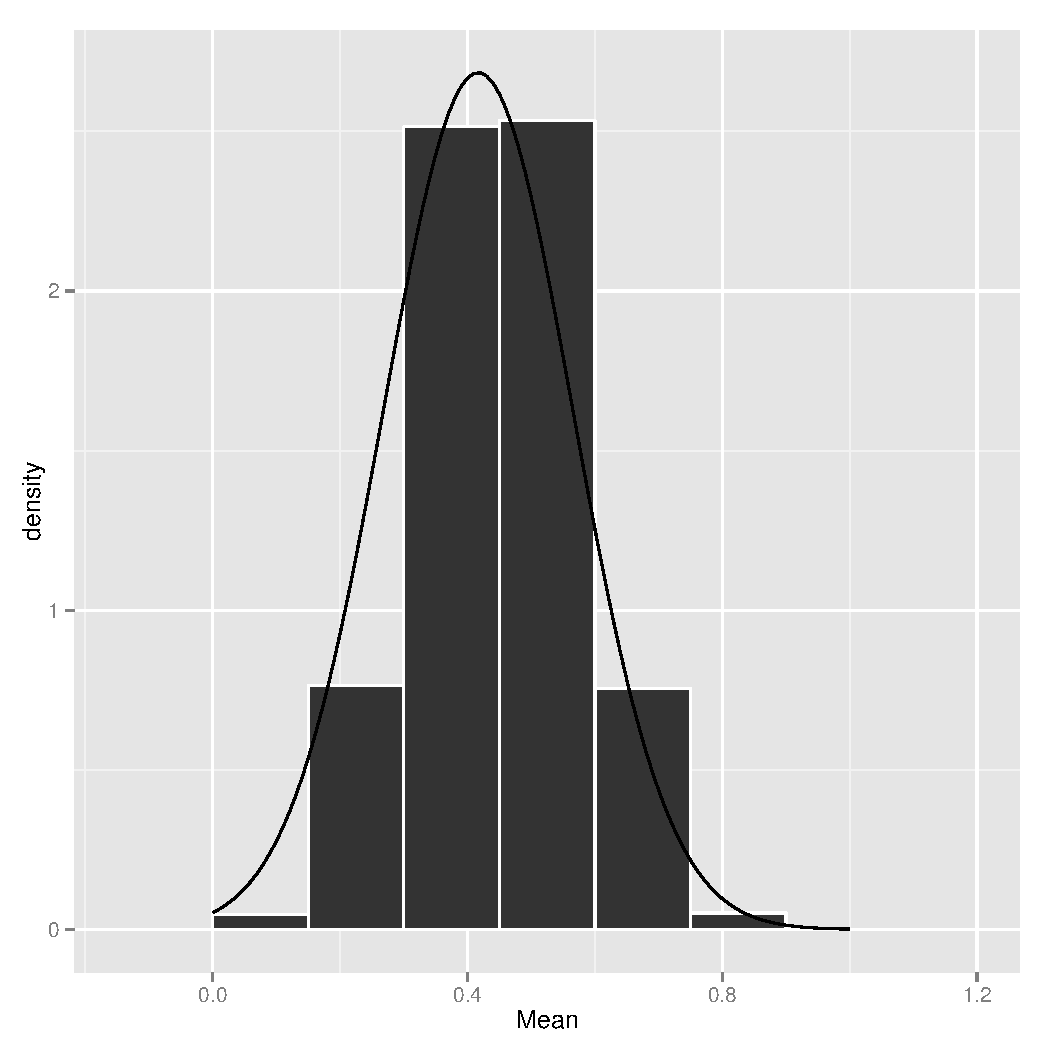
\includegraphics[width = .5\textwidth]{histogram_1e-1.pdf}
\caption{Histogram of 100,000 simulated values of the sample mean when the sample was taken without replacement from a box that contains 5 ``1'' tickets and 7 ``0'' tickets.}
\end{figure}

\noindent And the exact, empirical and approximated probabilities are given in the following table. Again we see that the Empirical estimation is extremely similar to the exact values, whereas the normal approximation is not nearly as accurate.

\begin{table}[H]
\centering
\begin{tabular}{|c|ccc|}
  \hline
z & Exact & EmpiricalEst & NormalApprox \\ 
  \hline
-4.00 & 0.00 & 0.00 & 0.00 \\ 
  -3.00 & 0.00 & 0.00 & 0.01 \\ 
  -2.00 & 0.01 & 0.01 & 0.07 \\ 
  -1.00 & 0.12 & 0.12 & 0.33 \\ 
  1.00 & 0.12 & 0.12 & 0.33 \\ 
  2.00 & 0.01 & 0.01 & 0.07 \\ 
  3.00 & 0.00 & 0.00 & 0.01 \\ 
  4.00 & 0.00 & 0.00 & 0.00 \\ 
   \hline
\end{tabular}
\caption{The exact value, empirical estimation and normal approximation of the tail probability for a box that contains 5 ``1'' tickets and 7 ``0'' tickets.} 
\end{table}






\pagebreak

 \section*{Question 2. Repeat (1) but with a box that contains 2 ``1" tickets and 98 ``0" tickets.}
 
 \subsection*{a) - d) with replacement}
Using the formulae we discussed in question 1,

$$E(\bar{X})= \frac{2}{100}$$ 
 
 $$SE(\bar{X}) = 0.057$$
 
 \noindent Both of which are significantly smaller than the values obtained in the previous question.\\ 

\noindent Next, we plot a histogram of 100,000 simulated $\bar{X}$ values as follows:
 
\begin{figure}[H]
\centering
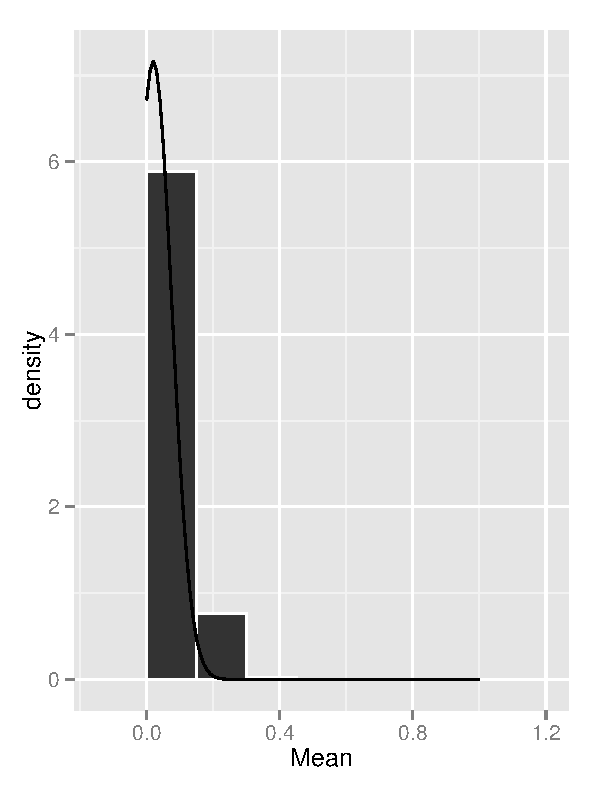
\includegraphics[width = .5\textwidth]{histogram_2c-1.pdf}
\caption{Histogram of 100,000 simulated values of the sample mean when the sample was taken with replacement from a box that contains 2 ``1" tickets and 98 ``0" tickets.}\label{q2}
\end{figure}
 
\noindent Finally, we calculate the exact, empirical and normal approximated probabilities:
\begin{table}[H]
\centering
\begin{tabular}{|c|ccc|}
  \hline
z & Exact & EmpiricalEst & NormalApprox \\ 
  \hline
-4.00 & 0.00 & 0.00 & 0.01 \\ 
  -3.00 & 0.00 & 0.00 & 0.06 \\ 
  -2.00 & 0.00 & 0.00 & 0.29 \\ 
  -1.00 & 0.00 & 0.00 & 0.68 \\ 
  1.00 & 0.11 & 0.12 & 0.68 \\ 
  2.00 & 0.11 & 0.12 & 0.29 \\ 
  3.00 & 0.01 & 0.01 & 0.06 \\ 
  4.00 & 0.01 & 0.01 & 0.01 \\ 
   \hline
\end{tabular}
\caption{The exact value, empirical estimation and normal approximation of the tail probability for a box that contains 2 ``1" tickets and 98 ``0" tickets.} 
\end{table}

\noindent As in question 1, the empirical estimation using the results of our simulated values nearly matches the probabilities. This time, the normal approximation is particularly bad. This is occurs because we only have two ``1" tickets in the box.  Figure~\ref{q2} shows that the empirical distribution of the sample mean is not even close to normal, as it is skewed right.  


\subsection*{e) without replacement}


\noindent Note that since we are now sampling without replacement, we have that
$$E(\bar{X})= \frac{2}{100}$$ 
$$SE(\bar{X}) = 0.056$$


\begin{figure}[H]
\centering
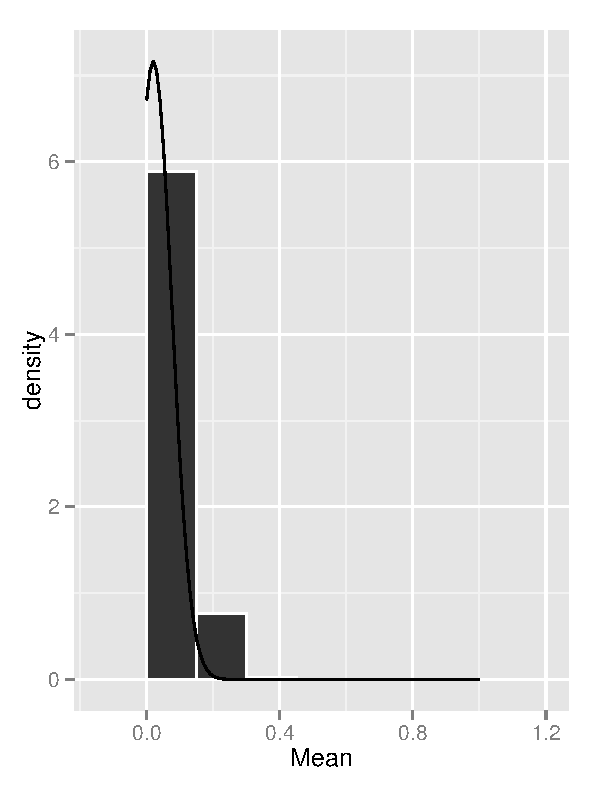
\includegraphics[width = .5\textwidth]{histogram_2e-1.pdf}
\caption{Histogram of 100,000 simulated values of the sample mean when the sample was taken without replacement from  a box that contains 2 ``1" tickets and 98 ``0" tickets.}
\end{figure}

\begin{table}[H]
\centering
\begin{tabular}{|c|ccc|}
  \hline
z & Exact & EmpiricalEst & NormalApprox \\ 
  \hline
-4.00 & 0.00 & 0.00 & 0.01 \\ 
  -3.00 & 0.00 & 0.00 & 0.07 \\ 
  -2.00 & 0.00 & 0.00 & 0.31 \\ 
  -1.00 & 0.00 & 0.00 & 0.69 \\ 
  1.00 & 0.12 & 0.12 & 0.69 \\ 
  2.00 & 0.12 & 0.12 & 0.31 \\ 
  3.00 & 0.00 & 0.00 & 0.07 \\ 
  4.00 & 0.00 & 0.00 & 0.01 \\ 
   \hline
\end{tabular}
\caption{The exact value, empirical estimation and normal approximation of the tail probability for a box that contains 2 ``1" tickets and 98 ``0" tickets.} 
\end{table}


\noindent Note that for this example, the results are extremely similar when the samples are taken both with and without replacement. Again we see that the normal approximation performs very poorly.


\pagebreak

 \section*{Question 3. Repeat (1) but with a box that contains tickets numbered ``1" to ``12".}
 
 \subsection*{a) - d) with replacement}
Using the formulae we discussed in question 1,

$$E(\bar{X})= 6.5$$ 
 
 $$SE(\bar{X}) = 1.409$$

 
\begin{figure}[H]
\centering
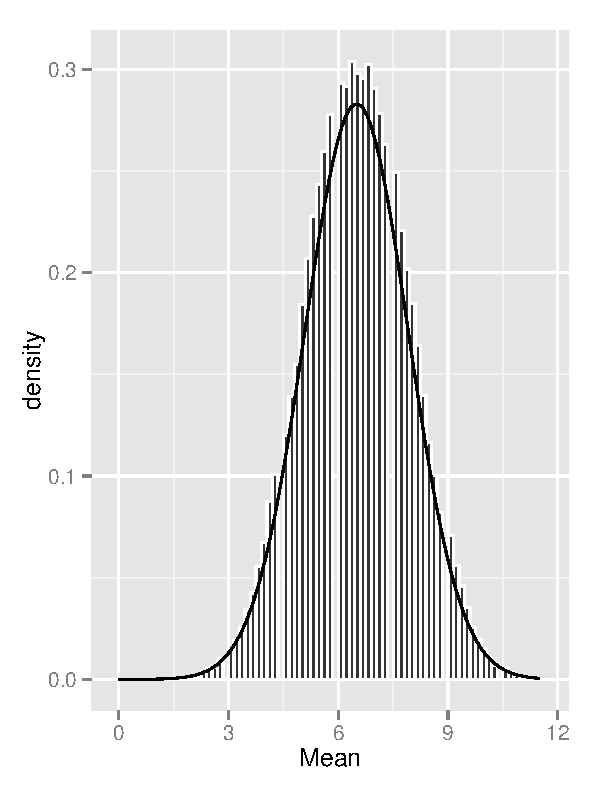
\includegraphics[width = .5\textwidth]{histogram_3c-1.pdf}
\caption{Histogram of 100,000 simulated values of the sample mean when the sample was taken with replacement from a box that contains tickets numbered ``1" to ``12".}\label{fig:q3c}
\end{figure}
 

\begin{table}[H]
\centering
\begin{tabular}{|c|cc|}
  \hline
z & EmpiricalEst & NormalApprox \\ 
  \hline
-4.00 & 0.00 & 0.00 \\ 
  -3.00 & 0.00 & 0.00 \\ 
  -2.00 & 0.02 & 0.03 \\ 
  -1.00 & 0.16 & 0.17 \\ 
  1.00 & 0.16 & 0.17 \\ 
  2.00 & 0.03 & 0.03 \\ 
  3.00 & 0.00 & 0.00 \\ 
  4.00 & 0.00 & 0.00 \\ 
   \hline
\end{tabular}
\caption{The exact value, empirical estimation and normal approximation of the tail probability for a box that contains tickets numbered ``1" to ``12".} \label{tab:q3c}
\end{table}

\noindent In this case, the values in the box have a discrete uniform distribution.  There are no ``outliers", so the normal approximation performs quite well (Figure~\ref{fig:q3c}, Table~\ref{tab:q3c}), even with the small sample size of $n=6$.



\subsection*{e) without replacement}


\noindent Note that since we are now sampling without replacement, we have that
$$E(\bar{X})= 6.5$$ 
$$SE(\bar{X}) = 1.041$$


\begin{figure}[H]
\centering
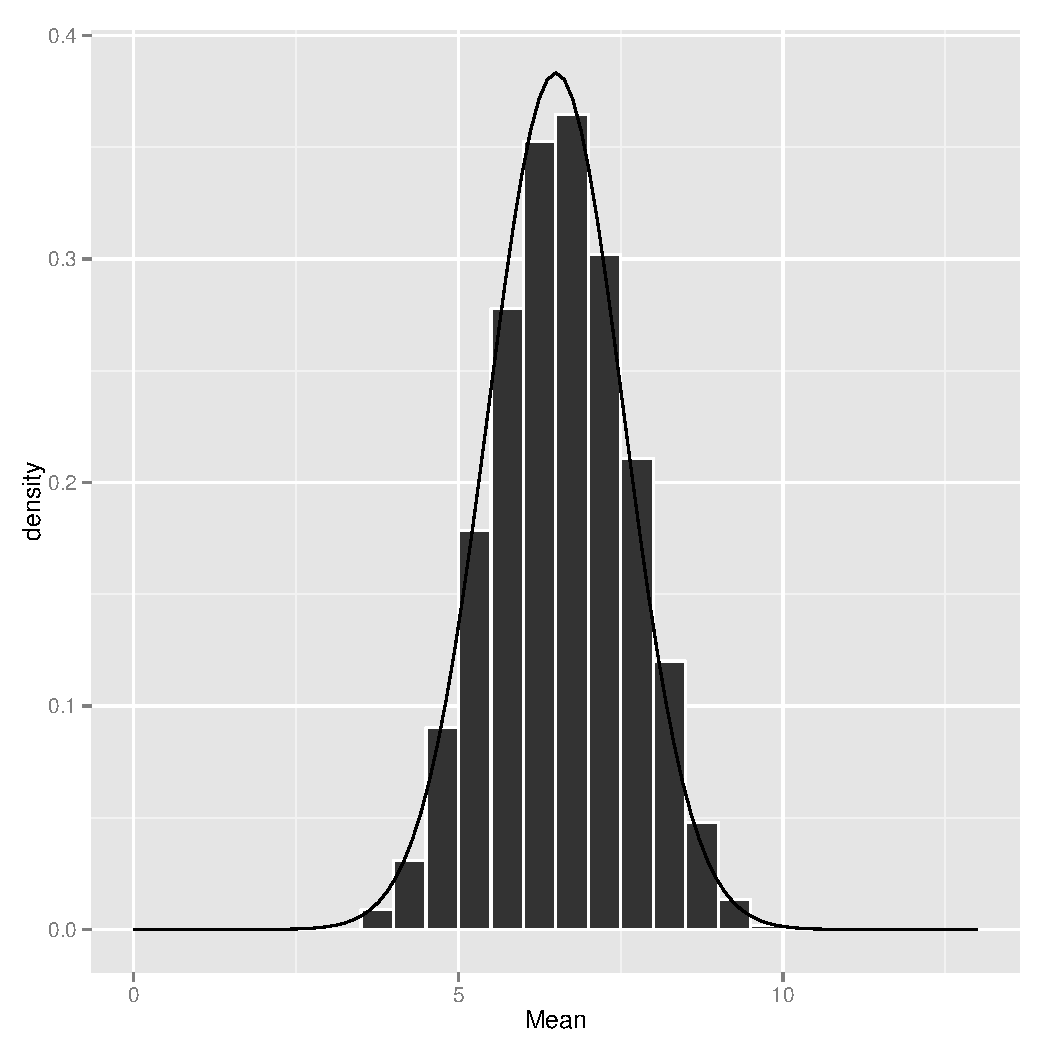
\includegraphics[width = .5\textwidth]{histogram_3e-1.pdf}
\caption{Histogram of 100,000 simulated values of the sample mean when the sample was taken without replacement from a box that contains tickets numbered ``1" to ``12".}
\end{figure}

\begin{table}[H]
\centering
\begin{tabular}{|c|cc|}
  \hline
z & EmpiricalEst & NormalApprox \\ 
  \hline
-4.00 & 0.00 & 0.00 \\ 
  -3.00 & 0.00 & 0.00 \\ 
  -2.00 & 0.02 & 0.03 \\ 
  -1.00 & 0.15 & 0.18 \\ 
  1.00 & 0.16 & 0.18 \\ 
  2.00 & 0.02 & 0.03 \\ 
  3.00 & 0.00 & 0.00 \\ 
  4.00 & 0.00 & 0.00 \\ 
   \hline
\end{tabular}
\caption{The exact value, empirical estimation and normal approximation of the tail probability for a box that contains tickets numbered ``1" to ``12".} 
\end{table}


\noindent When sampling without replacement in this instance, the normal approximation to the probabilities is not performing as well as when sampling with replacement, however the distribution of the $\bar{X}$'s does appear to be fairly normal.


\pagebreak

 \section*{Question 4. Repeat (1) but with a box that contains tickets numbered ``1" to ``11" and a ticket labelled ``30".}
 
 \subsection*{a) - d) with replacement}
Using the formulae we discussed in question 1,

$$E(\bar{X})= 8$$ 
 
 $$SE(\bar{X}) = 2.977$$

 
\begin{figure}[H]
\centering
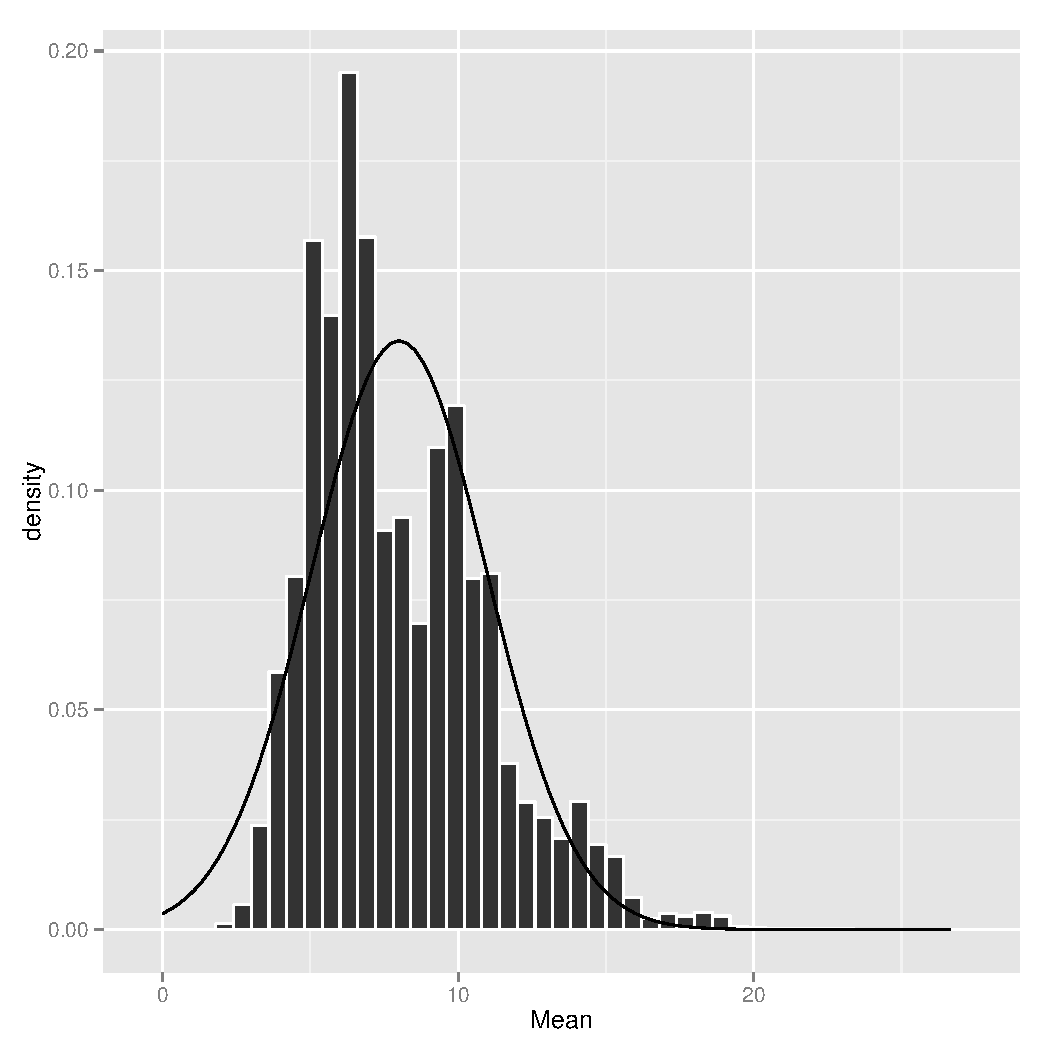
\includegraphics[width = .5\textwidth]{histogram_4c-1.pdf}
\caption{Histogram of 100,000 simulated values of the sample mean when the sample was taken with replacement from a box that contains tickets numbered ``1" to ``11" and a ticket labelled ``30".}\label{fig:q4c}
\end{figure}
 

\begin{table}[H]
\centering
\begin{tabular}{|c|cc|}
  \hline
z & EmpiricalEst & NormalApprox \\ 
  \hline
-4.00 & 0.00 & 0.00 \\ 
  -3.00 & 0.00 & 0.00 \\ 
  -2.00 & 0.00 & 0.02 \\ 
  -1.00 & 0.14 & 0.17 \\ 
  1.00 & 0.16 & 0.17 \\ 
  2.00 & 0.05 & 0.02 \\ 
  3.00 & 0.01 & 0.00 \\ 
  4.00 & 0.00 & 0.00 \\ 
   \hline
\end{tabular}
\caption{The exact value, empirical estimation and normal approximation of the tail probability for a box that contains tickets numbered ``1" to ``11" and a ticket labelled ``30".} \label{tab:q4c}
\end{table}

\noindent The outlier at $30$ makes the distribution of the sample mean skewed right and bimodal (Figure~\ref{fig:q4c}.  Thus, it makes little sense to use the normal approximation.  Table~\ref{tab:q4c} confirms this, as the normal approximation is bad at points not near the center of the distribution.



\subsection*{e) without replacement}


\noindent Note that since we are now sampling without replacement, we have that
$$E(\bar{X})= 8$$ 
$$SE(\bar{X}) = 2.198$$


\begin{figure}[H]
\centering
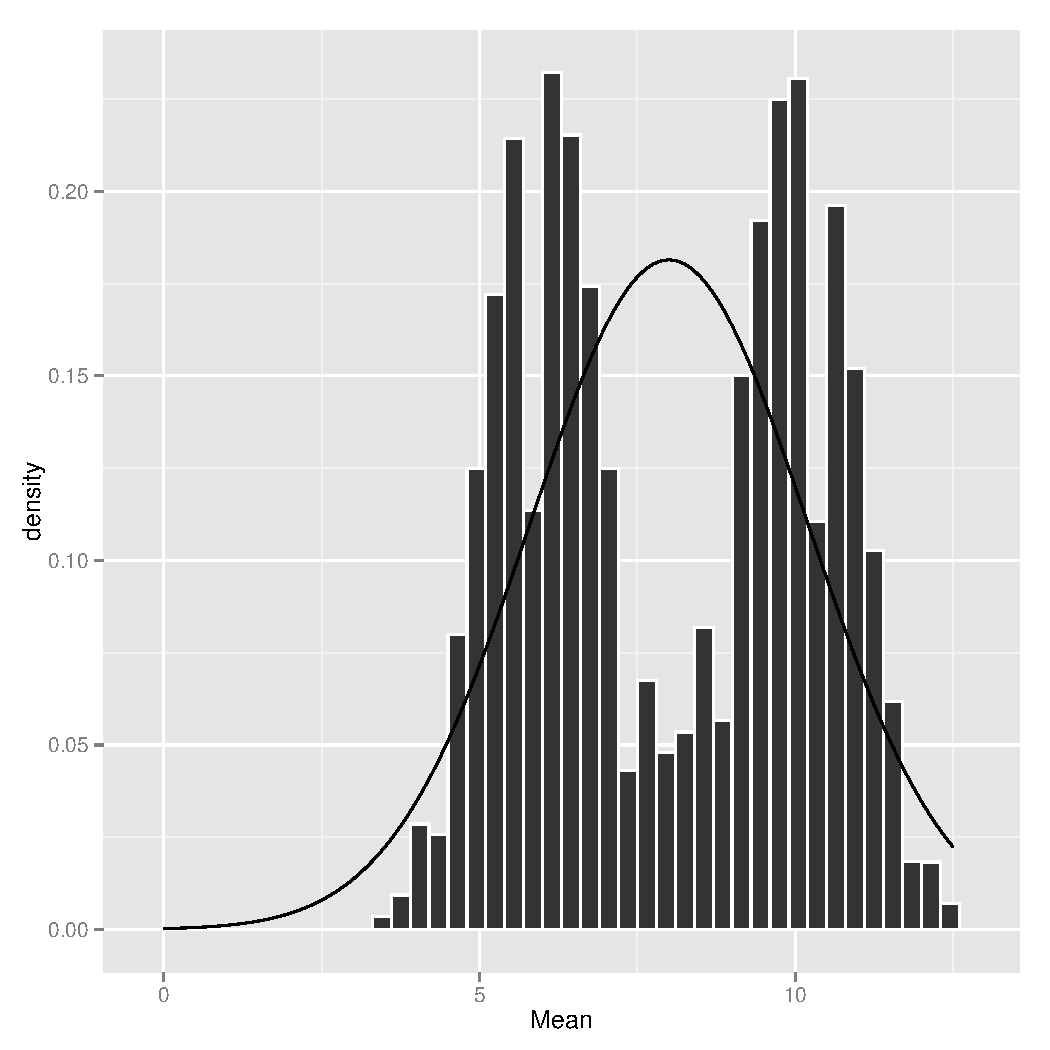
\includegraphics[width = .5\textwidth]{histogram_4e-1.pdf}
\caption{Histogram of 100,000 simulated values of the sample mean when the sample was taken without replacement from a box that contains tickets numbered ``1" to ``11" and a ticket labelled ``30".}\label{fig:q4e}
\end{figure}

\begin{table}[H]
\centering
\begin{tabular}{|c|cc|}
  \hline
z & EmpiricalEst & NormalApprox \\ 
  \hline
-4.00 & 0.00 & 0.00 \\ 
  -3.00 & 0.00 & 0.00 \\ 
  -2.00 & 0.00 & 0.02 \\ 
  -1.00 & 0.20 & 0.17 \\ 
  1.00 & 0.20 & 0.17 \\ 
  2.00 & 0.00 & 0.02 \\ 
  3.00 & 0.00 & 0.00 \\ 
  4.00 & 0.00 & 0.00 \\ 
   \hline
\end{tabular}
\caption{The exact value, empirical estimation and normal approximation of the tail probability for a box that contains tickets numbered ``1" to ``11" and a ticket labelled ``30".} \label{tab:q4e}
\end{table}


\noindent When sampling without replacement, the distribution of the sample mean becomes bimodal and appears roughly symmetric (Figure~\ref{fig:q4e}).  The normal approximation is a poor estimate here.


\pagebreak

\section*{Extra Credit}
\subsection*{Repeat for other boxes and sample sizes that you find interesting, and comment on what you learn. Along with boxes constructed ``by hand'' like those in (1)-(4), you may be interested to fill your box with tickets that have been randomly generated by sampling from various distributions (e.g. normal, exponential, log-normal.)}

We are interested in the box in question (4), which has discrete uniform observations from $1$ to $11$ and a single outlier at $30$.  Populations like this occur in real life all the time.  For example, we might be interested in the average number of dollars that somebody spent per purchase, where most purchases were small amounts but they made a few relatively large purchases. \\

\noindent We investigate how the normal approximation to the distribution of the sample mean improves as the sample size increases.  In question (4), we sampled 6 tickets from the box.  Here, we try sampling 8 and 10.  When sampling with replacement, the standard errors of the sample mean with $n=6, 8, 10$ are approximately $2.977, 2.578, 2.306$ respectively.  Without replacement, the standard errors are approximately $2.198,1.555$, and $0.983$.  This confirms our intuition that the sample mean becomes more concentrated around the true value of the box mean as the sample size increases.  Figure~\ref{fig:ec} shows that the distribution of the sample mean is bimodal for smaller $n$, but smooths out and appears more Gaussian as the sample size increases.

\begin{figure}[H]
\centering
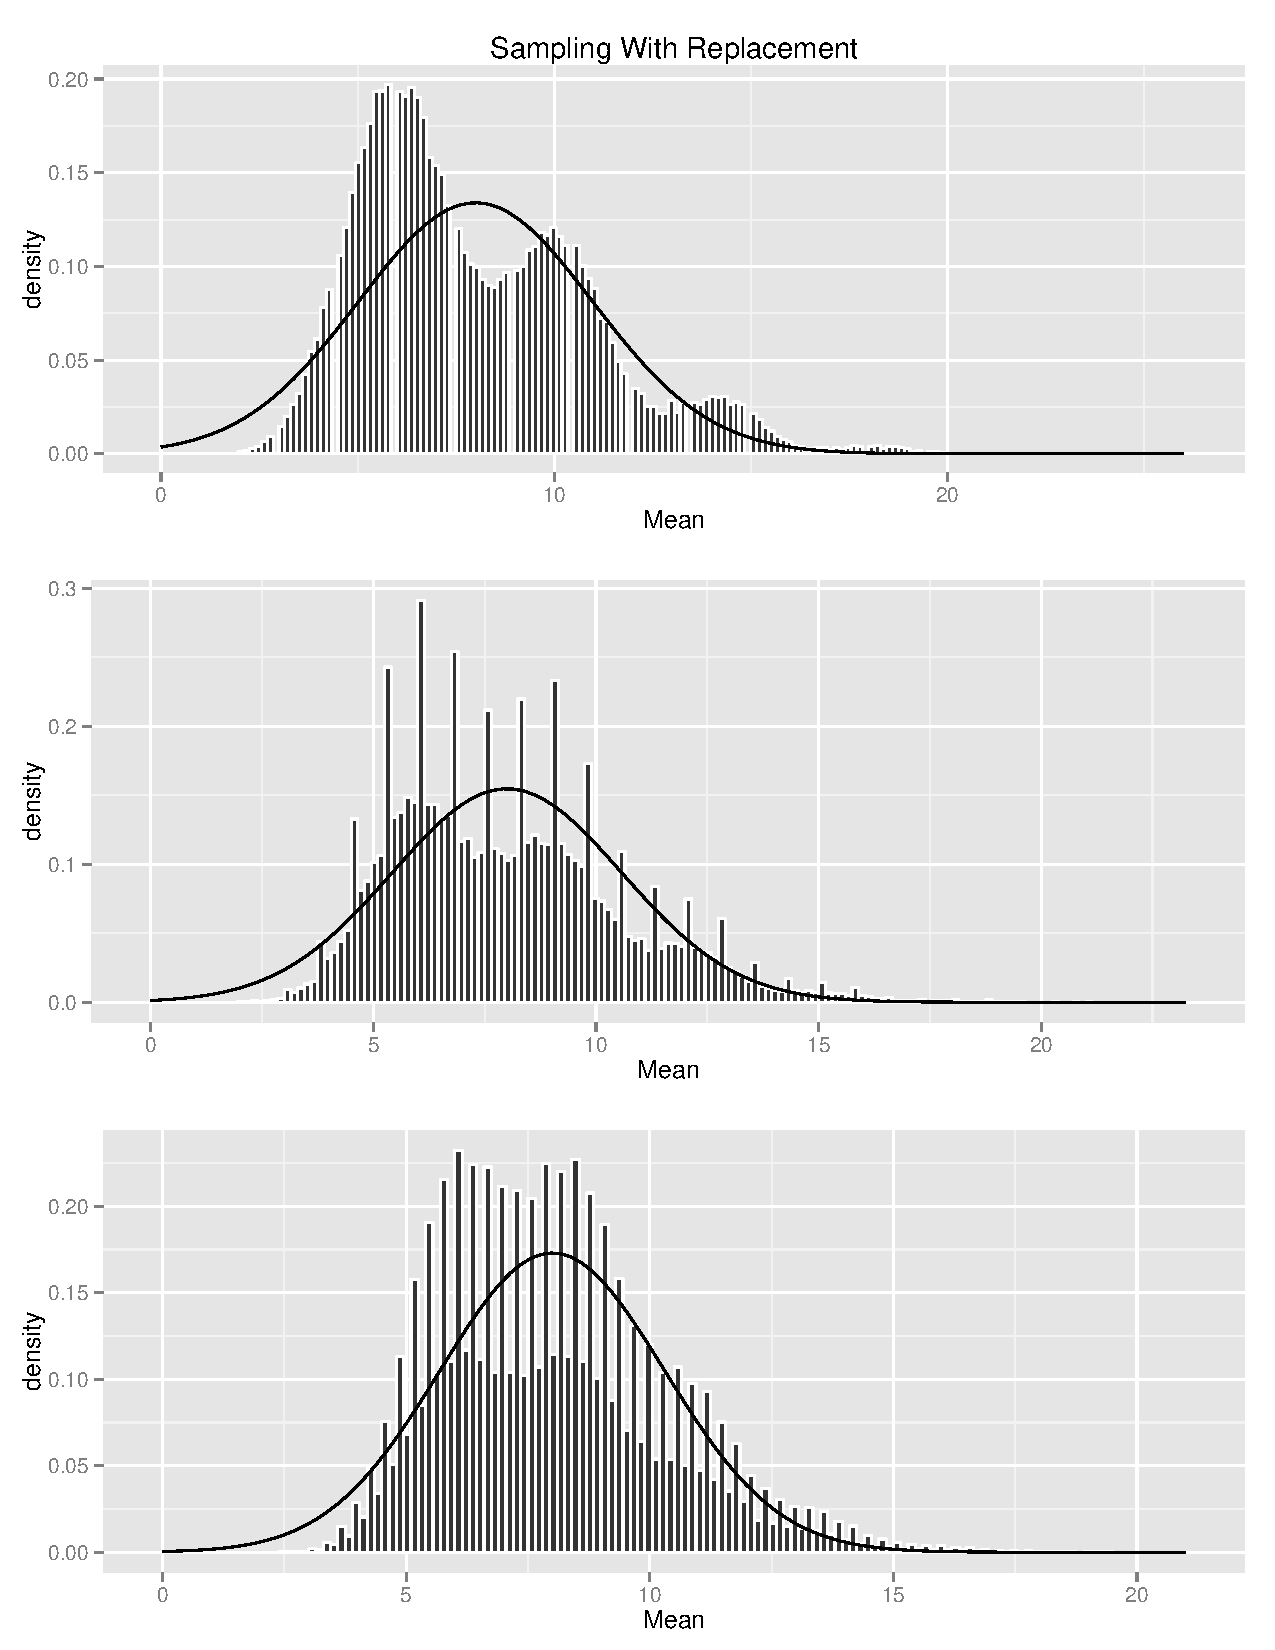
\includegraphics[width = .5\textwidth]{histogram_ec_wr.pdf}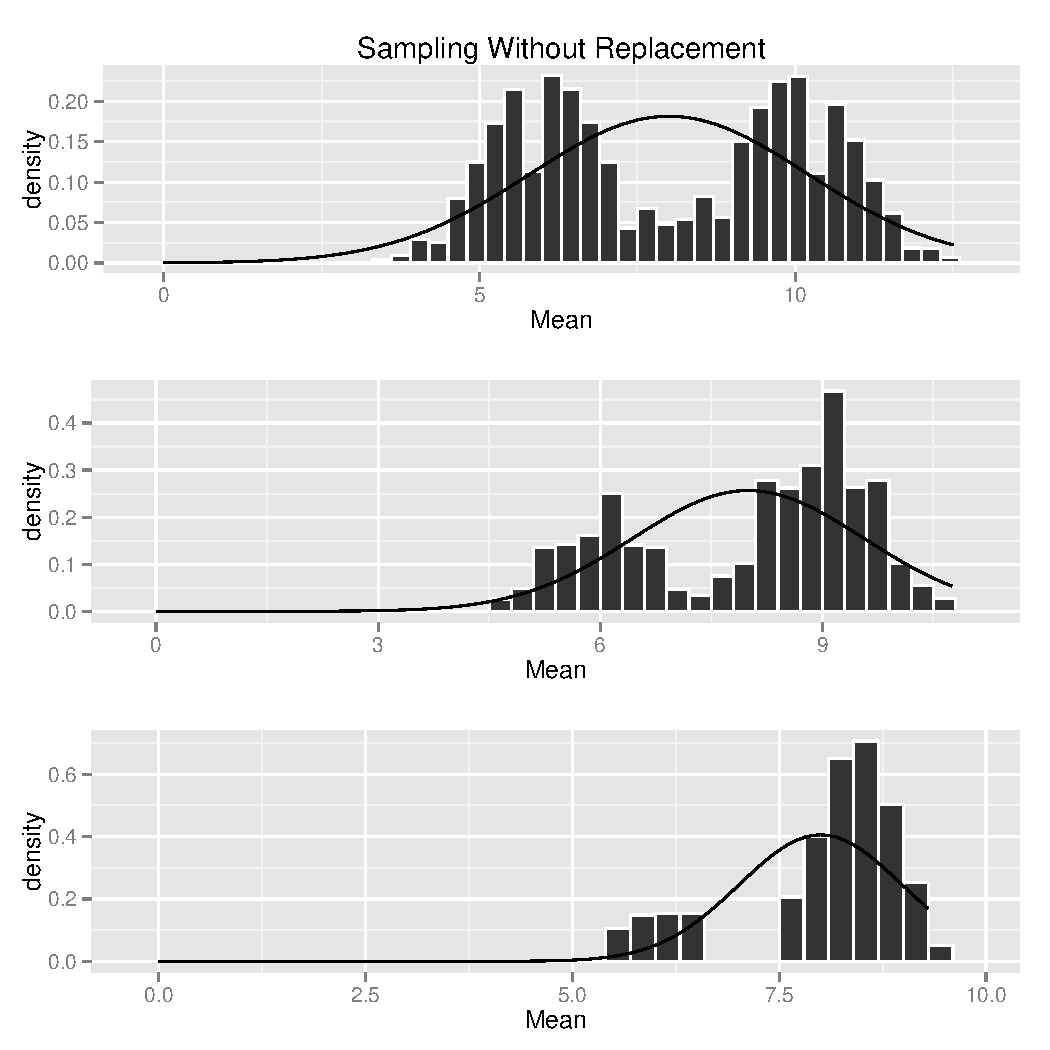
\includegraphics[width = .5\textwidth]{histogram_ec_nr.pdf}
\caption{Distribution of the sample mean, where rows represent sampling with $n=6, 8,$ and $10$.}\label{fig:ec}
\end{figure}


\pagebreak



\section*{Small Extra Credit}
\subsection*{In class we considered the model
$$Y=a+X$$
where $X$ is standard normal, and ask the question of whether $a^2$ is estimable. Is it? Justify your answer.}

We claim that $Y^2 - 1$ is an unbiased estimator of $a^2$. The proof is as follows:

\begin{align*}
E(Y^2 - 1) &= E(a^2 + 2aX + X^2 - 1) \\
&= E(a^2) + E(2aX) + E(X^2) + E(-1) \\
&= a^2 + 2aE(X) + E(X^2) - 1 \\
&= a^2 + 0 + (E(X)^2 + \text{Var}(X)) - 1 \\
&= a^2 + 0 + 1 - 1\\
&= a^2
\end{align*}

\end{document}
